\documentclass{perassignments}



\usepackage{hyperref}
\usepackage[abjad]{pertheorems}
\usepackage{mathtools}
\usepackage{amsmath}
\usepackage{float}
\usepackage{common}
\usepackage{xepersian}




\settextfont[]{XBNiloofar}
%\setmathdigitfont{XBTabriz}


\CourseName[آز شبکه‌]
\Semester[اول]
\Year[01]
\Prof[دکتر صفائی]
\Dept[دانشکده مهندسی کامپیوتر]
\CollabFirst[عماد زین‌اوقلی]{98103267}
\CollabSecond[پارسا رییسی]{98103223}
\CollabThird[سیدابوالفضل رحیمی ]{97105941}

\renewcommand{\maketitle}{\MakeMyLabTitle}
\allowdisplaybreaks


\begin{document}
	\maketitle
	\section{HTTP}
	سایت 
	\texttt{math.sharif.ir}
	باز کردیم و نتایج زیر 
	\ref{fig:1b}
	 را گرفتیم.
	\begin{figure}[H]
		\centering
		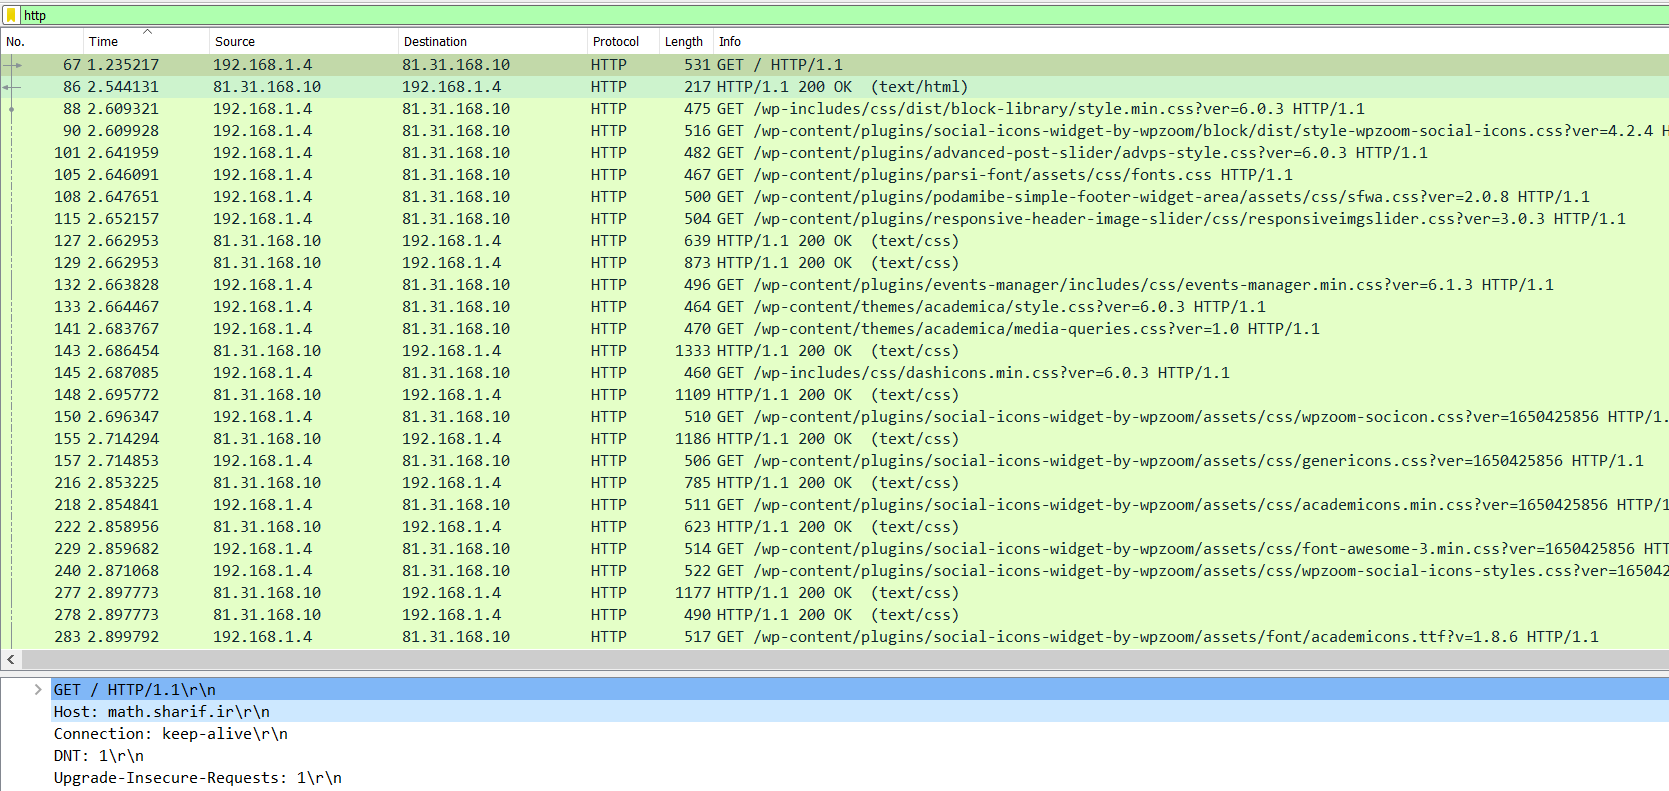
\includegraphics[width= 0.7\linewidth]{graphics/1a.png}
		\caption{فیلتر بر حسب پروتکل HTTP}
		\label{fig:1a}
	\end{figure}
	\begin{enumerate}
		\item 
		ابزار آماری wireshark خروجی زیر
		\ref{fig:1b}
		 را داده است.
		\begin{figure}[H]
			\centering
			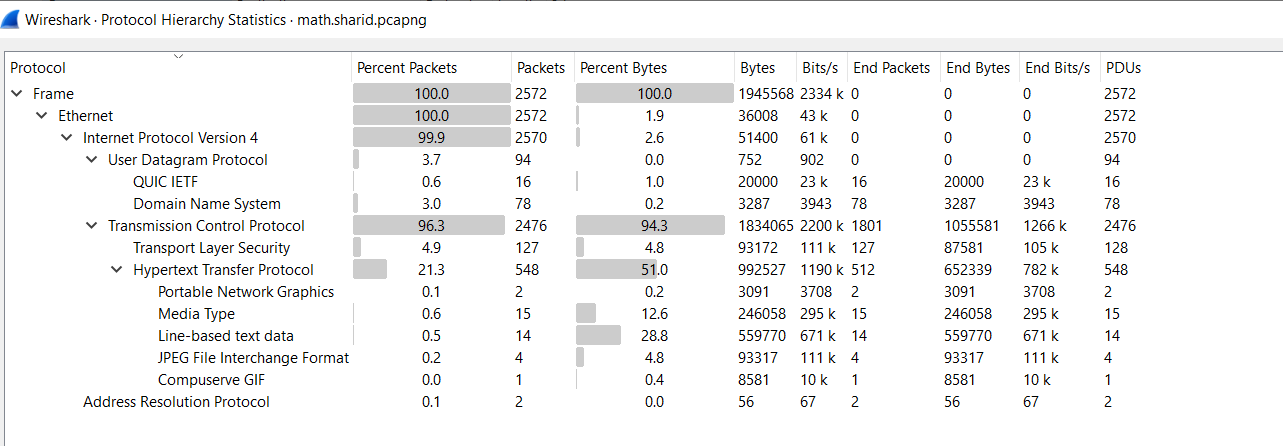
\includegraphics[width= 0.7\linewidth]{graphics/1b.png}
			\caption{تفکیک بر اساس پروتکل‌ها}
			\label{fig:1b}
		\end{figure}
		\item 
		با توجه به 
		\ref{fig:1b}
		فاصله زمانی بین درخواست تا پاسخ برابر با 
		\(1.3\)
		ثانیه بوده است.
		\item 
		ابتدا بایستی چک‌باکس 
		\lr{relative sequence number}
		در 
		\lr{preferences}
		را خاموش کنیم. سپس با توجه به 
		\ref{fig:1c}
		شماره اولین درخواست TCP برابر با 
		\texttt{606236787}
		است. 
		\begin{figure}[H]
			\centering
			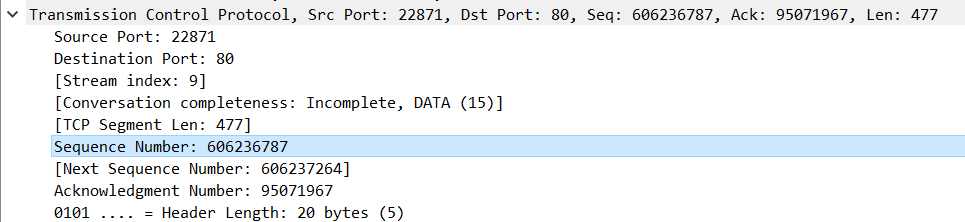
\includegraphics[width= 0.7\linewidth]{graphics/1c.png}
			\caption{اولین درخواست TCP}
			\label{fig:1c}
		\end{figure}
		\item
		با فیلتر کردن بر حسب پروتکل DNS 
		\ref{fig:1d}
		در می‌یابیم که اکثر درخواست‌ها از نوع A بوده است.
		\begin{figure}[H]
			\centering
			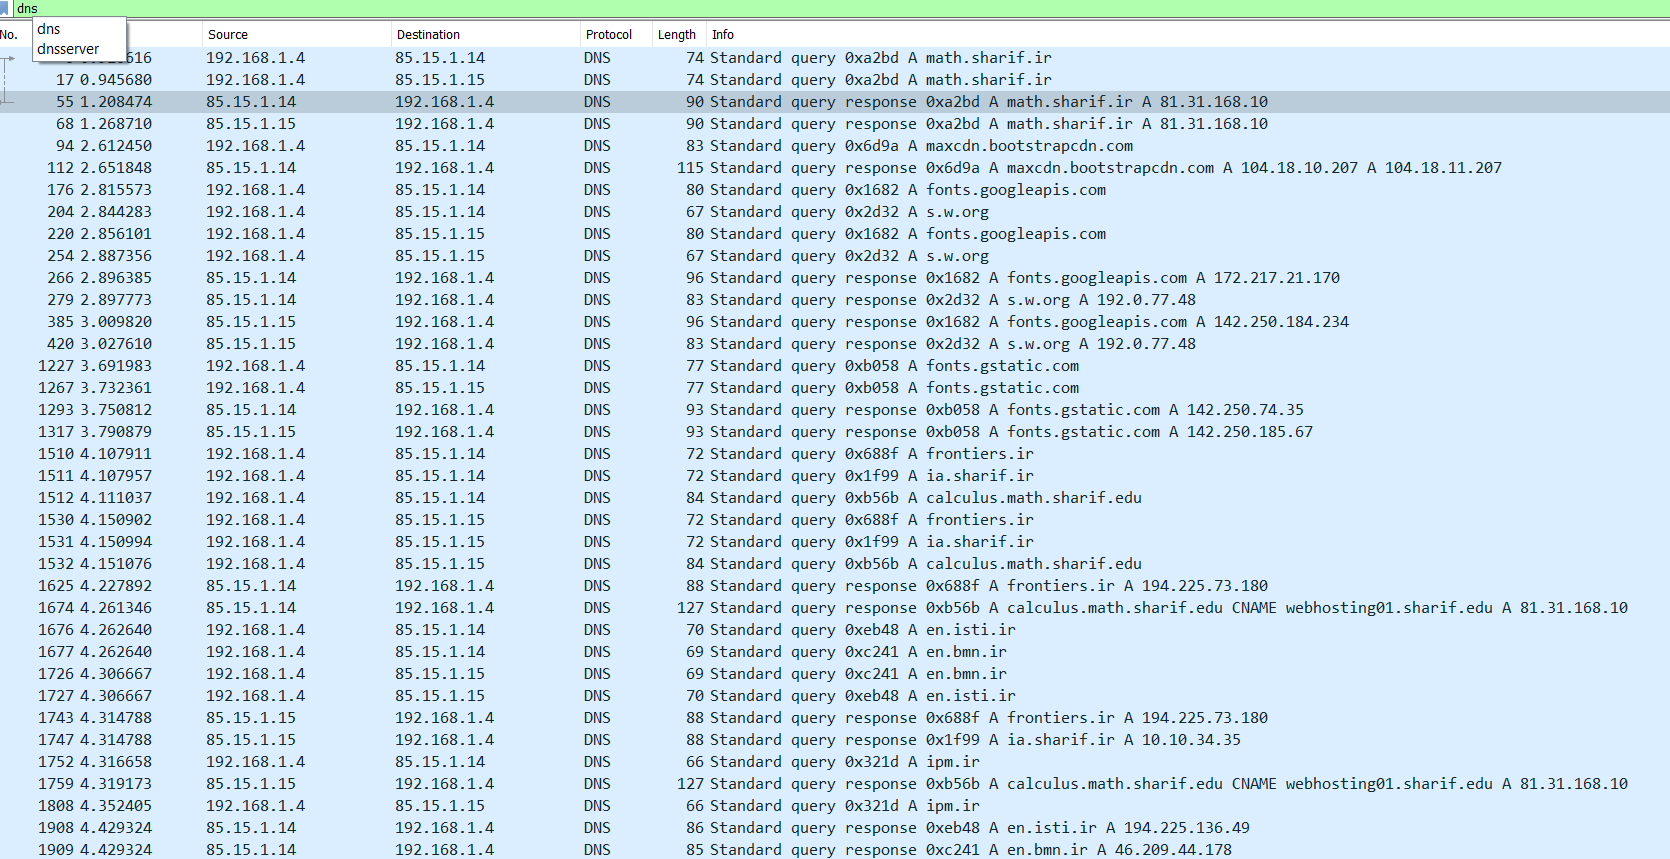
\includegraphics[width= 0.7\linewidth]{graphics/1d.png}
			\caption{فیلتر بر حسب پروتکل DNS}
			\label{fig:1d}
		\end{figure}
		\item 
		گزینه 
		\lr{\texttt{Export Objects: HTTP}}
		را از منو 
		\ref{fig:1e}
		 انتخاب می‌کنیم.
		 \begin{figure}[H]
		 	\centering
		 	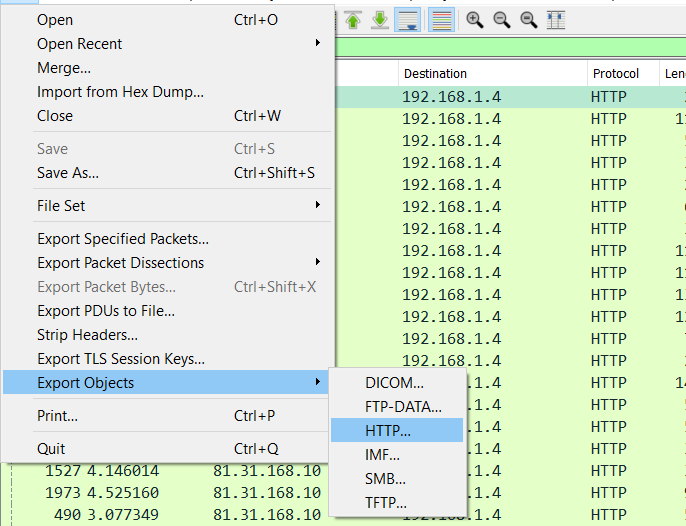
\includegraphics[width= 0.7\linewidth]{graphics/1e.png}
		 	\caption{\lr{\texttt{Export Objects: HTTP}}}
		 	\label{fig:1e}
		 \end{figure}
	 	دو نمونه زیر را انتخاب کردیم.
	 	 \begin{figure}[H]
	 		\centering
	 		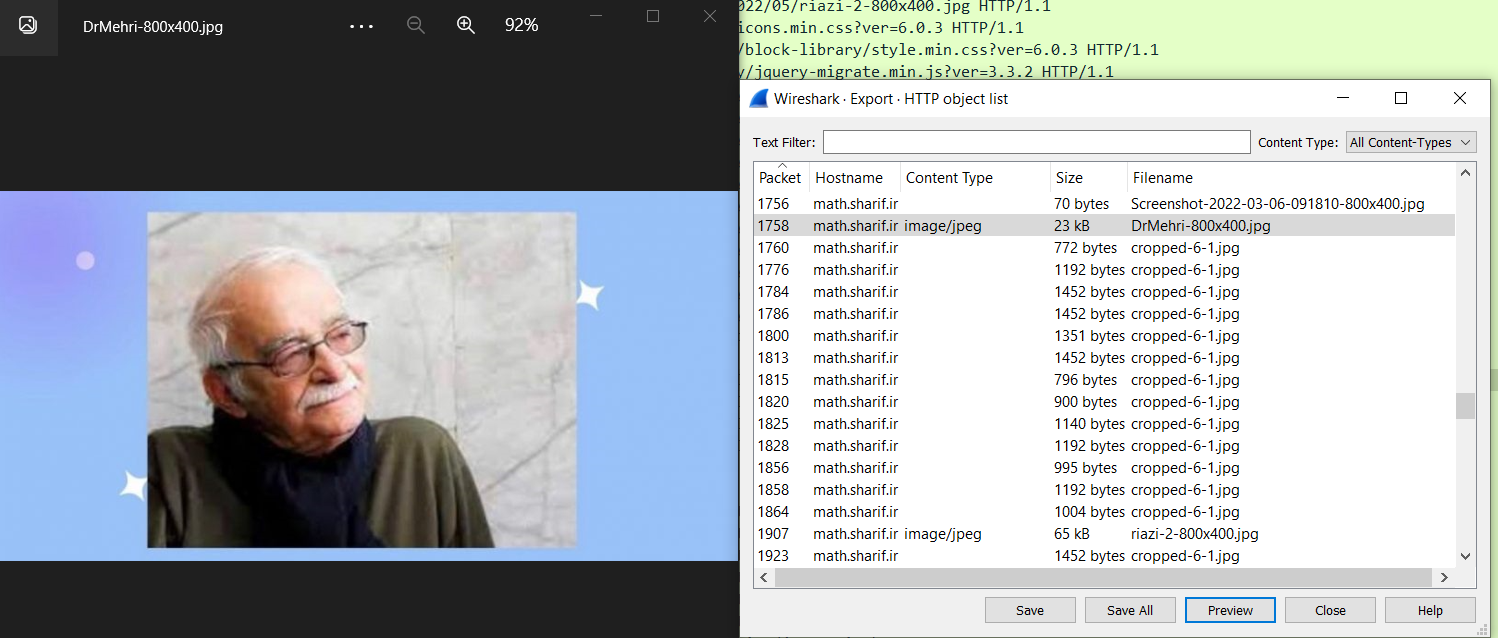
\includegraphics[width= 0.7\linewidth]{graphics/1f.png}
	 		\caption{نمونه اول}
	 		\label{fig:1f}
	 	\end{figure}
 	 \begin{figure}[H]
 		\centering
 		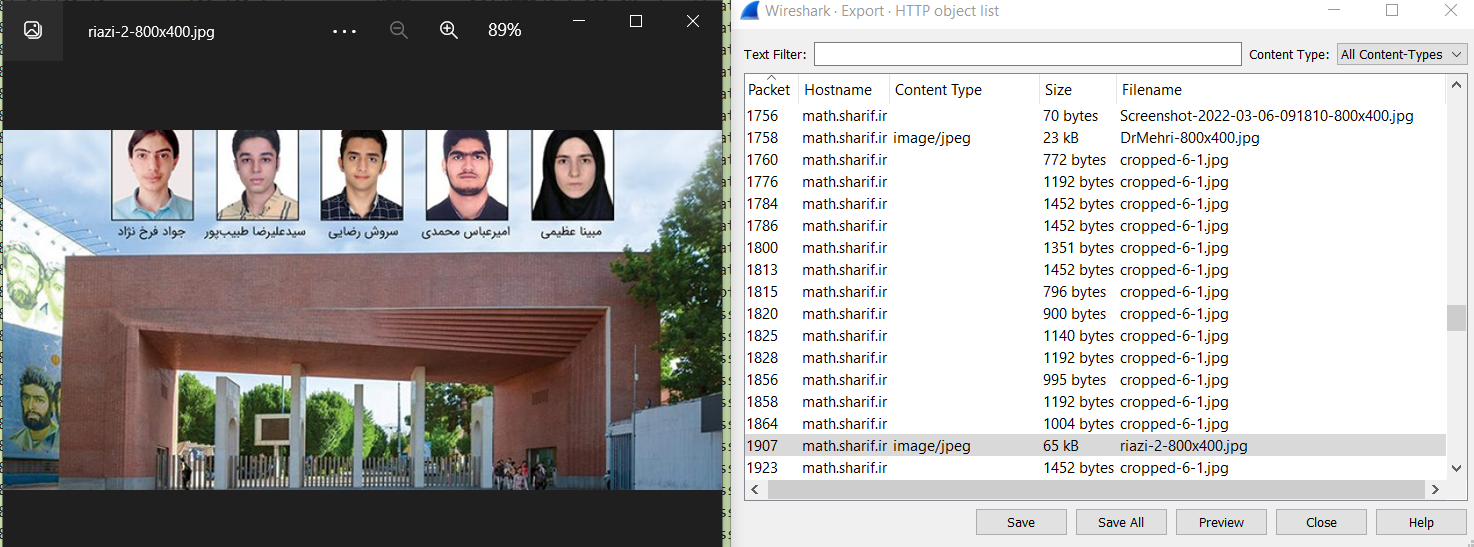
\includegraphics[width= 0.7\linewidth]{graphics/1g.png}
 		\caption{نمونه دوم}
 		\label{fig:1g}
 	\end{figure}
	\end{enumerate}
	\section{Telnet}
	
	\begin{enumerate}
		\item
		با توجه به جواب DNS می‌فهمیم که IP آدرس سرور 
		\texttt{64.13.139.230}
		و آدرس کلاینت 
		\texttt{192.168.1.4}
		است.
		\begin{figure}[H]
			\centering
			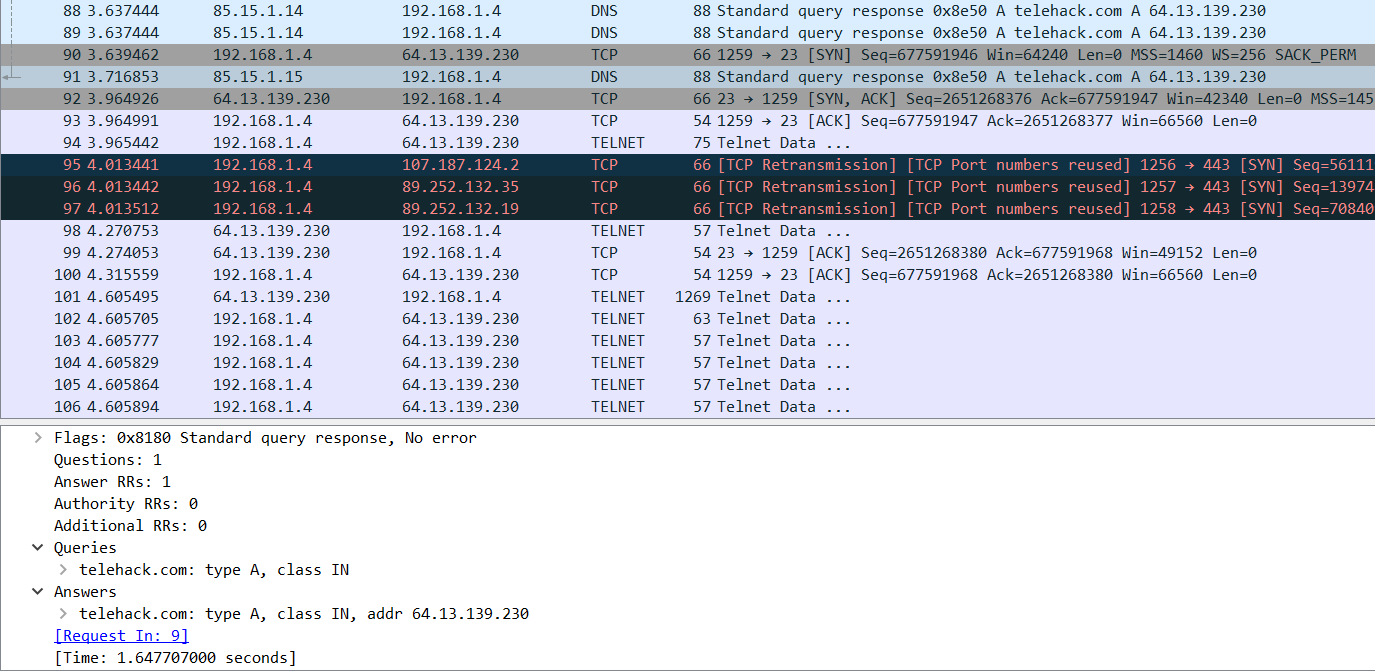
\includegraphics[width= 0.7\linewidth]{graphics/2a.png}
			\caption{\lr{IP Address}}
			\label{fig:2a}
		\end{figure}
		\item 
		با استفاده از قابلیت 
		\lr{Follow TCP Stream}
		\ref{fig:2b} 
		می‌توان حرف فرستاده و گرفته شده را مشاهده کرد.
		\begin{figure}[H]
			\centering
			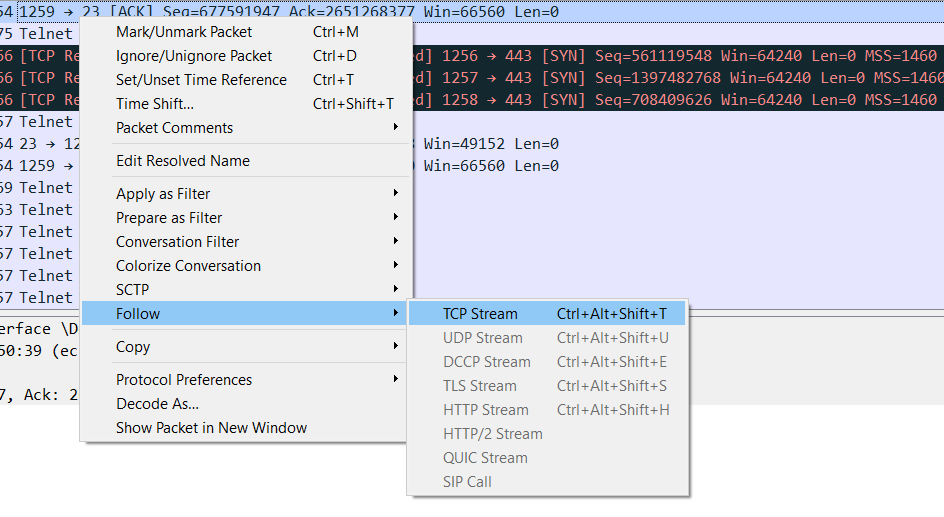
\includegraphics[width= 0.7\linewidth]{graphics/2b.png}
			\caption{\lr{Follow TCP Stream}}
			\label{fig:2b}
		\end{figure}
	\begin{figure}[H]
		\centering
		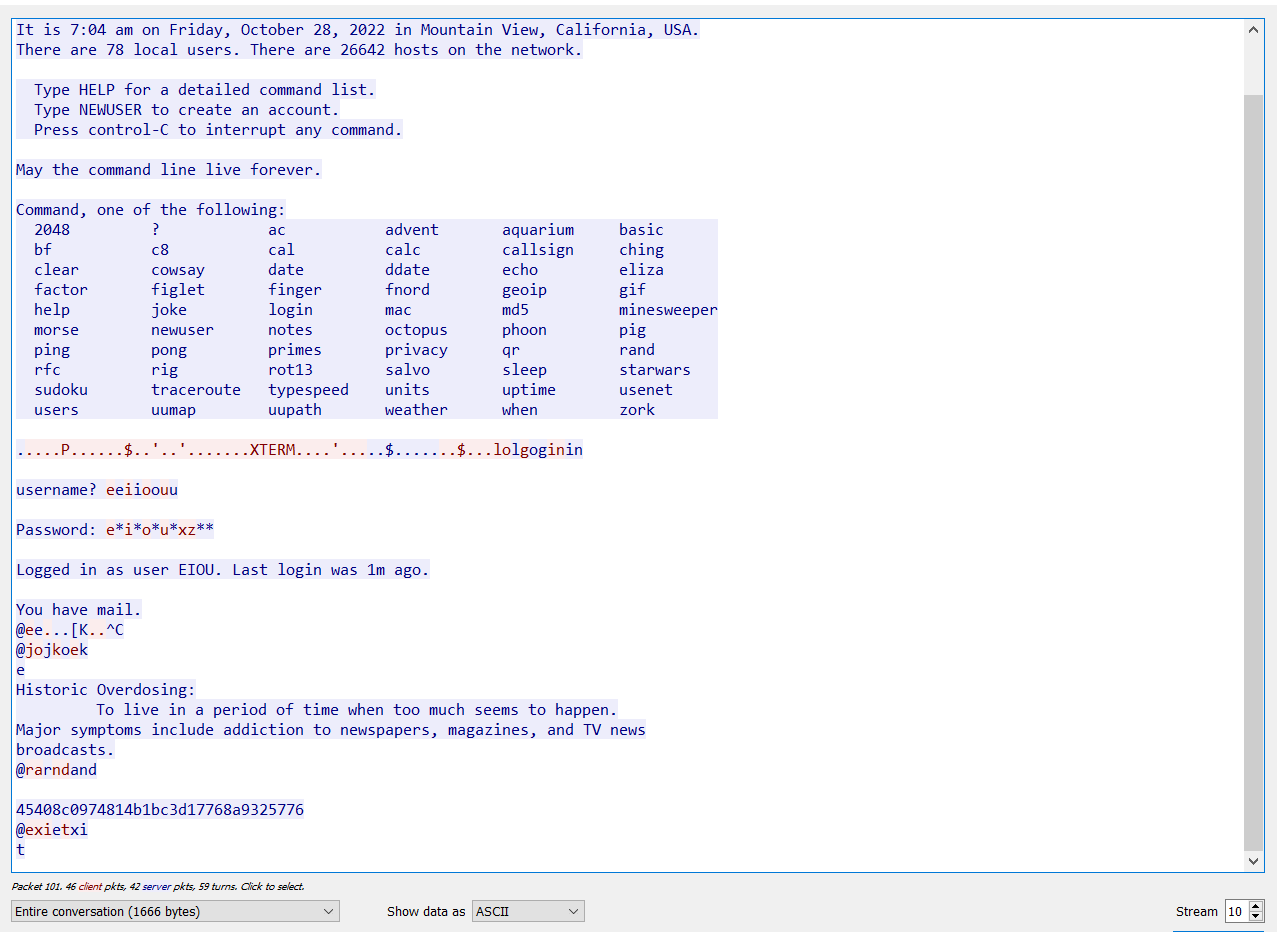
\includegraphics[width= 0.7\linewidth]{graphics/2c.png}
		\caption{ارتباط Telnet}
		\label{fig:2c}
	\end{figure}
	مشاهده می‌کنیم که 
	\lr{\texttt{username: eiou}}
	و 
	\lr{\texttt{password: eiouxz}}
	است. 
	\item 
	با توجه به 
	\ref{fig:2c}
	دستورات فرستاده شده 
		\texttt{login}, \texttt{joke}, \texttt{rand}, \texttt{exit}
	بودند.
	\end{enumerate}
	\section{DNS}
	آزمایش را با سایت 
	\texttt{sharif.ir}
	انجام دادیم.
		\begin{figure}[H]
		\centering
		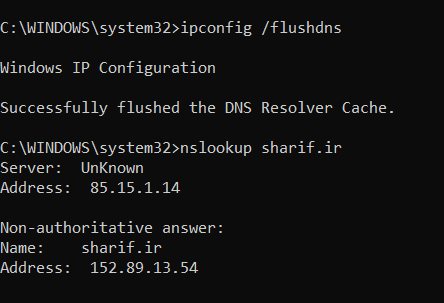
\includegraphics[width= 0.7\linewidth]{graphics/3a.png}
		\caption{\lr{\texttt{nslookup sharif.ir}}}
		\label{fig:3a}
	\end{figure}
	\begin{figure}[H]
	\centering
	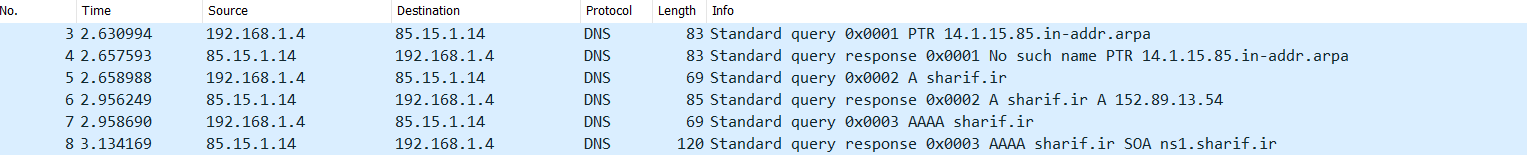
\includegraphics[width= 0.7\linewidth]{graphics/3d.png}
	\caption{فیلتر برحسب DNS}
	\label{fig:3d}
\end{figure}
	
	\begin{enumerate}
		\item
		با توجه به 
		\ref{fig:3a} 
		و
		\ref{fig:3d}
		در می‌یابیم که درخواست‌ها به و پاسخ‌ها از سرور 
		\texttt{85.15.1.14}
		ارسال می‌شوند.
		\item 
		هدر‌های درخواست و پاسخ DNS به صورت زیر 
		\ref{fig:3b},\ref{fig:3c}
		هستند. 
				\begin{figure}[H]
			\centering
			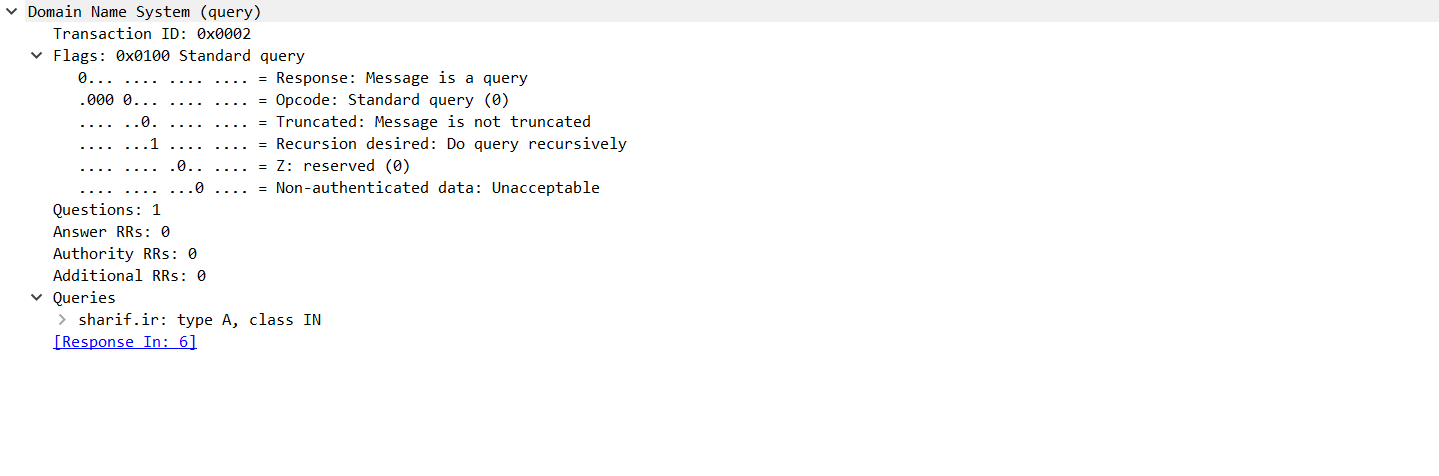
\includegraphics[width= 0.7\linewidth]{graphics/3b.png}
			\caption{درخواست DNS}
			\label{fig:3b}
		\end{figure}
		flag‌
		های هدر به ترتیب مشخص شده‌اند:
		\begin{description}
			\item [نوع پیام]
			این پیام یک درخواست است.
			\item [نوع درخواست]
			یک درخواست استاندارد است.
			\item [پیام خرد شده است؟]
			خیر، زیرا درخواست بزرگ نبوده است.
			\item[درخواست بازگشتی]
			بله درخواست به صورت بازگشتی حل شود.
		\end{description}
		سپس تعداد درخواست‌ها و غیره مشخص شده‌اند. در نهایت، درخواست‌مان آمده است که از نوع A یعنی 
		\lr{host address}
		و کلاس IN
		یعنی 
		\lr{internet}
		است. 
		\begin{figure}[H]
			\centering
			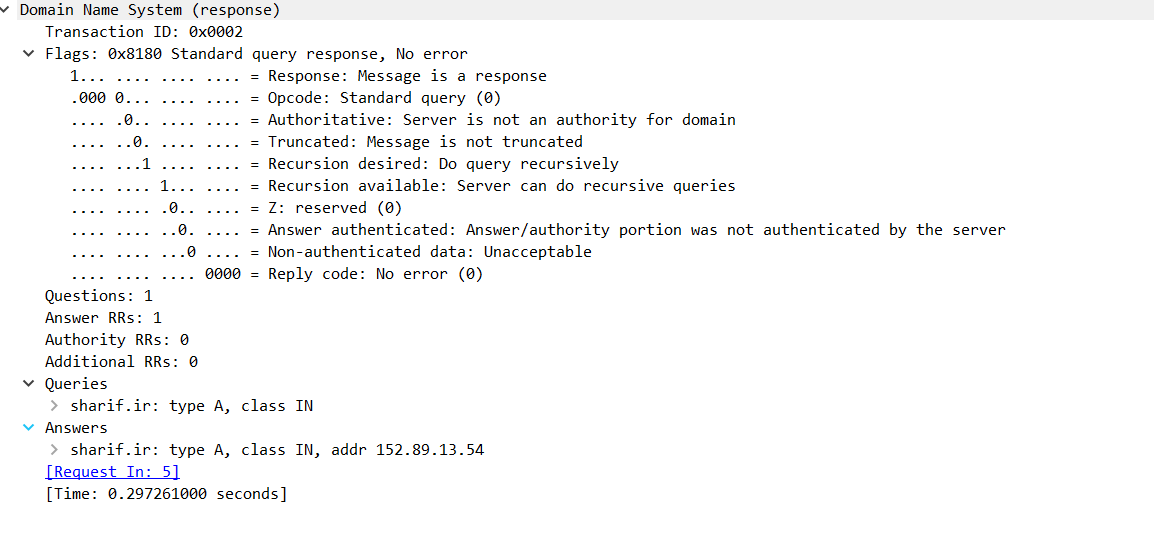
\includegraphics[width= 0.7\linewidth]{graphics/3c.png}
			\caption{پاسخ DNS}
			\label{fig:3c}
		\end{figure}
			flag‌
		های هدر به ترتیب مشخص شده‌اند:
		\begin{description}
			\item [نوع پیام]
			این پیام یک پاسخ است.
			\item [نوع درخواست]
			یک درخواست استاندارد است.
			\item [آیا سرور Authoritative است؟]
			خیر.
			\item [پیام خرد شده است؟]
			خیر، زیرا پاسخ بزرگ نبوده است.
			\item[درخواست بازگشتی]
			بله درخواست به صورت بازگشتی حل شود.
			\item[امکان درخواست بازگشتی]
			بله سرور می‌تواند درخواست به صورت بازگشتی حل کند.
		\end{description}
		سپس تعداد درخواست‌ها و غیره مشخص شده‌اند. در نهایت، درخواست‌مان و پاسخ آن آمده است که از نوع A و کلاس IN است و آدرس آن 
		\texttt{152.89.13.54}
		است. 
	\end{enumerate}
\end{document}